\documentclass[onecolumn, draftclsnofoot,10pt, compsoc]{report}

%slightly modified from stackoverflow @ https://tex.stackexchange.com/questions/200437/numbering-sections-subsections-etc-manually
%code block below allows for references to function as a section instead of a chapter
\makeatletter
\renewenvironment{thebibliography}[1]
{\subsection{References}
	\@mkboth{\MakeUppercase\bibname}{\MakeUppercase\bibname}%
	\list{\@biblabel{\@arabic\c@enumiv}}%
	{\settowidth\labelwidth{\@biblabel{#1}}%
		\leftmargin\labelwidth
		\advance\leftmargin\labelsep
		\@openbib@code
		\usecounter{enumiv}%
		\let\p@enumiv\@empty
		\renewcommand\theenumiv{\@arabic\c@enumiv}}%
%	\sloppy
	\clubpenalty4000
	\@clubpenalty \clubpenalty
	\widowpenalty4000%
	\sfcode`\.\@m}
{\def\@noitemerr
	{\@latex@warning{Empty `thebibliography' environment}}%
	\endlist}
\makeatother

\usepackage{graphicx}
\usepackage{url}
\usepackage{setspace}
\makeindex
\usepackage{geometry}
\usepackage{minitoc}
\usepackage{titlesec}

\titleformat{\chapter}[display]
{\normalfont\bfseries}{}{0pt}{\Huge}

\setcounter{minitocdepth}{1}
\setcounter{tocdepth}{0}

\geometry{textheight=9.5in, textwidth=7in}

% 1. Fill in these details
\def \CapstoneTeamName{		Wheelchair Data Collection Team}
\def \CapstoneTeamNumber{		4}
\def \GroupMemberOne{			Marie Bomber}
\def \GroupMemberTwo{			Aaron Leondar}
\def \GroupMemberThree{			Hadi Rahal-Arabi}
\def \CapstoneProjectName{			Robotic Wheelchair Data Collection and Analysis}
\def \CapstoneSponsorCompany{	Oregon State University}
\def \CapstoneSponsorPerson{	Matthew William Shuman	}

% 2. Uncomment the appropriate line below so that the document type works
\def \DocType{	%Problem Statement
				%Requirements Document
				%Technology Review
				%Design Document
					Final Report
				}
			
\renewenvironment{abstract}{%
	\hfill\begin{minipage}{0.95\textwidth}
		\rule{\textwidth}{1pt}}
	{\par\noindent\rule{\textwidth}{1pt}\end{minipage}}

\bibliographystyle{ieeetran}	
\newcommand{\NameSigPair}[1]{\par
\makebox[2.75in][r]{#1} \hfil 	\makebox[3.25in]{\makebox[2.25in]{\hrulefill} \hfill		\makebox[.75in]{\hrulefill}}
\par\vspace{-12pt} \textit{\tiny\noindent
\makebox[2.75in]{} \hfil		\makebox[3.25in]{\makebox[2.25in][r]{Signature} \hfill	\makebox[.75in][r]{Date}}}}
% 3. If the document is not to be signed, uncomment the RENEWcommand below
%\renewcommand{\NameSigPair}[1]{#1}

%%%%%%%%%%%%%%%%%%%%%%%%%%%%%%%%%%%%%%%
\begin{document}
\begin{titlepage}
    \pagenumbering{gobble}
    \begin{singlespace}
        \hfill 
        % 4. If you have a logo, use this includegraphics command to put it on the coversheet.
        %\includegraphics[height=4cm]{CompanyLogo}   
        \par\vspace{.2in}
        \centering
        \scshape{
            \huge CS Capstone \DocType \par
            {\large 12 June 2018}\par
            \vspace{.5in}
            \textbf{\Huge\CapstoneProjectName}\par
            \vfill
            {\large Prepared for}\par
            \Huge \CapstoneSponsorCompany\par
            \vspace{5pt}
            {\Large\NameSigPair{\CapstoneSponsorPerson}\par}
            {\large Prepared by }\par
            Group\CapstoneTeamNumber\par
            % 5. comment out the line below this one if you do not wish to name your team
            \CapstoneTeamName\par 
            \vspace{5pt}
            {\Large
                \NameSigPair{\GroupMemberOne}\par
                \NameSigPair{\GroupMemberTwo}\par
                \NameSigPair{\GroupMemberThree}\par
            }
            \vspace{20pt}
\begin{abstract}
% Add Abstract
				\end{abstract} 
        } 
    \end{singlespace}
\end{titlepage}
\newpage
\pagenumbering{arabic}
\dominitoc
\tableofcontents
%\listoffigures
%\listoftables
\clearpage


\chapter{Introduction to Project}
\minitoc
\section{Project Context}
Project Chiron, an OSU venture, has developed a prototype kit for allowing those with extreme disabilities to interact with Permobil wheelchairs. While the software and hardware is existing, Project Chiron lacks an interface for data collection and analysis. Our project aims to allow for simple recording of trial data, as well as organizing the data for analysis. Furthermore, there is little documentation on the custom kit that can be mounted on wheelchairs, so it is necessary to document the applications and usage instructions of the kit as we interact with it.
\\\\
The prototype hardware has several sets of sensors that have the capability of constantly collecting data. It will be necessary to develop an understanding of the value of the data collected from each sensor; the data may need to be truncated, or collected at set intervals.
\\\\
Presenting the data in a usable format for analysis provides an entirely different challenge. While data collection will require some understanding of what each sensor is measuring, data analysis and formatting will require an intimate understanding of the purpose of each measurement, as well as the implications of those measurements.
\section{Relevant People \& Roles}
\begin{center}
	\begin{tabular}{ c|c }
		Matthew Shuman & The client. Supervised and provided requirements to the project\\
		Marie Bomber & Group Member. Acted as project manager and systems developer     \\
		Aaron Leondar & Group Member. Provided style to front-end of project\\
		Hadi Rahal-Arabi & Group Member. Back-end programmer for the project server  \\
				
	\end{tabular}
\end{center}

\chapter{Requirements Document}
\minitoc
	\section{Introduction}
	\subsection{Purpose}
	This requirements document is intended to define the critical features and functionality for a GUI based testing interface for ROS. It is intended to act as an agreement between the client Matthew Shuman and the developers, Marie Bomber, Aaron Leondar and Hadi Rahal-Arabi (and any other relevant stakeholders) to the promised functions and abilities of the testing interface. 
	\subsection{Scope}
	The intent of this project is to produce a general purpose interface to design and run tests on robots that run ROS. Within this scope is a specific use-case of an easy to use interface for Project Chiron research. This interface will  begin and record user tests, and allow testing data to be retrieved so a researcher can run POMDP analysis on the gathered results. This project will not cover the modifications made to the Project Chiron robot (a Perimobile wheelchair) and will not include any hardware work with the exception of documenting any already-existing hardware modifications. 
	
	\subsection{Definitions, Acronyms and Abbreviations}
	\begin{description}
		\item [Researcher] \hfill \break Admin level user of the Robot Test Controller. The researcher is expected to have full access to all user testing data (including names)
		\item [POMDP] \hfill \break Partially Observable Markov Decision Process. Per POMDP.org "This is a mathematical model that can capture the domain dynamics that include uncertainty in action effects and uncertainty in perceptual stimuli. Once a problem is captured as POMDP, it them becomes more amendable for solution using optimization techniques." \cite{1}
		\item [ROS] \hfill \break Robot Operating System
		\item [ROS Bag] \hfill \break Collection of ROS Topic data created by the ROSbag library during a user test
		\item [ROS Topics] \hfill \break A feature of ROS that 'publishes' relevant robot data and one of the primary communication methods of ROS. \cite{3} Examples of ROS Topics include the movement of a robotic arm or the contents of a video camera 'eye'. 
		\item [Tester] \hfil \break Mid level user of the Robot Test Controller. The tester is expected to be able to initiate a user test, but will not be able to retrieve all user data. (May be able to retrieve data via an ID, but will not have access to testee names).
		\item [Test Participant] \hfill \break Individual who has no access to the Robot Testing Controller, but will have a name and/or ID entry and who will run a user test.
		\item [User Test] \hfill \break Instance of a single navigation of the testing course. This test will produce a bag of test participant data that the Robot Test Controller must be able to store and retrieve.
	\end{description}
	\bibliography{Bibliography}
	\subsection{Overview}
	This software requirements specification document contains all of the constraints of the robot test controller. It can be used as a functional description for the necessary components of the project, without discussion of their design or implementation.
	
	
	\section{Overall Description}
	\subsection{Product Perspective}
	\begin{itemize}
		\item Interactions with the robot to be tested must be done with ROS, as it is a standard of the parent project.
		\item There will be no development or addition of hardware, only documentation of existing Project Chiron hardware.
	\end{itemize}
	\subsection{Product Functions}
	\subsubsection{Create a New Test}
	\begin{itemize}
		\item The application must allow a researcher to create and name a new test
		\item Once the robot is selected, the application must populate available ROS topics on the robot
		\item The researcher must be able to enter the following testing data
		\subitem The IP of the robot to be tested
		\subitem Where the researcher would like test information to be stored
		\subitem What ROS topics to record
		\subitem What metadata to include in the test
		\subitem The names of test participants or the number of participants in the test
		\item Once topics are selected, the interface should provide an estimate of how large a ROSbag would be based on selected topics. This estimate must be in a size per minute of test format
	\end{itemize}
	\subsubsection{Run an Existing Test}
	\begin{itemize}
		\item The application must allow a user to select and run a test based on the definitions of a previously created test
		\item Once the test is selected the tester must be able to select which test participant to record data under. This can be an ID or test participant name, based on the test definitions
		\item The tester must be able to select which test number to record (to allow a test participant to be tested multiple times)
		\item The application must report the current connection status to the robot
		\item The application must auto-populate metadata when possible (such as date/time of test)
		\item The application must report a test status, such as 'waiting to begin', 'initializing' or 'begin'.
		\item The application must allow the tester to begin and end tests.
	\end{itemize}
	\subsubsection{Export Test Data}
	\begin{itemize}
		\item The researcher should be able to see a list of bags, sortable by trial date/time and name or ID of testee.
		\item It must be simple to replace names associated with bags with testee IDs, to maintain data integrity but provide confidentiality to the testers.
		\item The core system should be able to accept a collected bag and correlate it with input from the user interface to create a data entry.
		\subitem The system should recognize if the user entered is a new testee or previous testee and link the new test to previous information.
		\item When passed a request from the user interface, the core system should pass the query to the main storage medium and return from the query in a format that meets the User Interface needs.
		\item The core system should securely store user logins and accept login requests so the interface only requires to handle pass/no pass scenarios.
	\end{itemize}
	\subsubsection{Wheelchair to Application Communication}
	\begin{itemize}
		\item Application must connect with the wireless network of the robot.
		\item Application must be able to collect the list of tasks that the robot has available
		\item The bags, when stored, must also have relevant metadata. Examples of metadata include:
		\subitem The length of time of the trial.
		\subitem The date and time the trial was performed.
		\subitem the ID of the participant.
	\end{itemize}
	\subsubsection{Data Storage}
	\begin{itemize}
		\item The system must recognize two levels of user access.
		\subitem Researcher - This level will have full access to user data, including test participant name and/or ID link.
		\subsubitem This level will also be able to delete the link between test participant name and test data at the researchers discretion
		\subitem Tester - This level has the ability to enter a testee name and start and end a test, but not have access to bag data.
	\end{itemize}
	\subsubsection{System Documentation}
	\begin{itemize}
		
		\item Wiring for the testing hardware must be diagrammed so that the system could be recreated. 
		\item Structure of hardware system documentation must be at a level that an electrical engineer can recreate the system
		\subitem Once documentation is completed, it must meet researcher satisfaction
		\item All system software must be documented so a software engineer can install and run the application on a new system with no issues. 
		\subitem To test, software must be installed by 3 senior software engineering students in a new environment without error. 
	\end{itemize}
	\subsection{User Characteristics}
	\begin{itemize}
		\item The user of the recording interface will be an unaffiliated paid undergraduate student, as such the collector must have a simple button interface for recording data.
		\item The users receiving the bag will be researchers affiliated with the robotic research, as such access to the bags should be trivial, but authenticated
		
	\end{itemize}
	\subsection{Constraints}
	\begin{itemize}
		\item The data entry must be stored in a secure storage space that complies with the Institutional Review Board as defined by the client.
		\subitem Testee names must be separate from a unique ID.
		\subitem The reference link between testee names and ID's must be able to be purged at the client's request.
		\item All testing hardware must be recorded with part numbers and pricing.
		\item The tester should experience little latency (less than 500ms) when sorting bags in the interface.
		\item The researcher must have a method of exporting bags, or accessing bags outside of the interface.
		\item The interface must be portable, both capable of running externally on a server, or locally.
		\item Bags cannot contain more than strictly required data because all bags must fit on a moderately-sized flash drive (no more than 16GB).
	\end{itemize}
	\subsection{Assumptions and Dependencies}
	\begin{itemize}
		\item Changes to the parent project may impact requirements of the robot test collector interface.
		\item The bag files should be appropriately sized to facilitate portable storage of roughly 100 trial runs.
		\begin{figure}[h!]
			
			\centering
			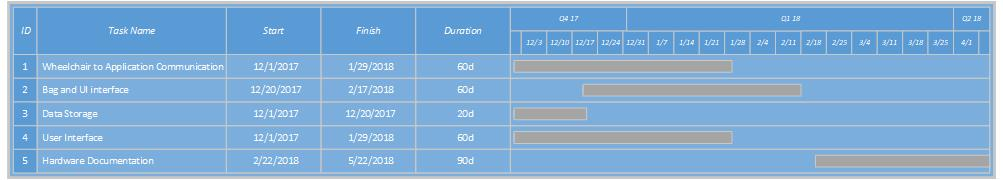
\includegraphics[width=\linewidth, scale=0.7]{PrelimGanttChart.jpg}
			Figure 1. The deadlines above are dependent on The Project Chiron research timeline
		\end{figure}
		
	\end{itemize}
	


\chapter{Design Document}
\minitoc

\section{Introduction}
This document provides a high-level view of the robot test interface project, broken up into four conceptual layers. Marie Bomber has designed the project management layer, as well as the storage layer. Aaron Leondar has developed a design for the communication layer. Lastly, Hadi Rahal-Arabi has created a design for the user interface. These four layers have been designed to meet specifications provided by Matthew Shuman.

\subsection{Glossary}
\begin{description}
	\item [Bag] \hfill \break File format used in ROS for storing ROS message data
	\item [POMDP] \hfill \break Partially Observable Markov Decision Process. Per POMDP.org "This is a mathematical model that can capture the domain dynamics that include uncertainty in action effects and uncertainty in perceptual stimuli. Once a problem is captured as POMDP, it them becomes more amendable for solution using optimization techniques."  \cite{POMDP}
	\item Project Chiron \hfill \break A research project from Oregon State University's Personal Robotics Group focused on increasing the mobility of people with extreme disabilities\cite{Chiron}. 
	\item [Raspberry Pi] \hfill \break A credit card sized single-board computer. Project Chiron uses the Raspberry Pi to manage the wheelchair sensors and ROS installed.
	\item [Research Participant] \hfill \break Individual who has no access to the Robot Test collection interface, but will have a name and/or ID entry within the interface. Their role is to participate in one or more test sessions with Project Chiron.
	\item [Researcher] \hfill \break Admin level user of the Robot Test Collection interface. The researcher is expected to have full access to all user testing data (including names)
	\item [ROS] \hfill \break Robot Operating System
	\item [Tester] \hfil \break Mid level user of the Robot Test Collection Interface. The tester is expected to be able to initiate a user test, but will not be able to retrieve all user data.
	\item [User Test] \hfill \break Instance of a single navigation of the testing course. This test will produce a bag of testee data that the Chiron interface must be able to store and retrieve.
	
\end{description}
\subsection{Design Stakeholders}
The stakeholders for this project are as follows:
\begin{description}
	\item Professor Matthew Shuman - Client and primary researcher of Project Chiron.
	\item Benjamin Nathan Narin - Graduate Student and additional researcher of Project Chiron.
	\item Marie Bomber - Member of the Robotic Wheelchair Data Collection and Analysis Senior Capstone Team
	\item Aaron Leondar - Member of the Robotic Wheelchair Data Collection and Analysis Senior Capstone Team 
	\item Hadi Rahal-Arabi - Member of the Robotic Wheelchair Data Collection and Analysis Senior Capstone Team
	\item Testers - Student employee running the Robot Test Collection interface once completed
	\item Research Participants - Student research participant who will be using Project Chiron to navigate a predefined test course.
\end{description}
\section{Organization and Project Management}
\subsection{Overview}
Because the project includes three distinct design layers that will need to interact with complex ways, we have decided to include a project manager role to manage scheduling and delegation of tasks. This section will focus on the technologies to aid in project management as well as outlining responsibilities of the project manager's role. 
\subsection{Design Concerns}
When defining and delegating tasks, any tools used must allow for both high level and detailed explanation of the task. Integration between tools is also required, to help track project flow and proactively identify design issues. The project manager will need to be able to break down requirements into reasonable chunks and prioritize tasks with respect to application dependencies. The team is using an agile approach and therefore will need a project 'scrum' board, a version control system and a communication channel. 
\subsection{Design Elements}
To manage delegation of tasks, we have selected the waffle.io as our scrum board. It will allow the program manager to quickly create and delegate tasks, as well as add issue notes to either add user stories (to define a component in the system) or clarify the requirements of the task. Waffle.io was chosen because it integrates smoothly with public github repos so as components are added, their code can be stored on a separate branch and the task will be automatically moved to complete once the code is merged. Similarly, slack has been selected as the primary project communication channel, it integrates with waffle.io so updates are posted as tasks are moved, and files can easily be uploaded to store client meeting notes or share project information that does not easily store in git (such as PDFs). The project manager will be responsible for creating and delegating project tasks, whether they be related to development or classroom assignments. In addition, they will be responsible for ensuring the initial version of the application is available to the client in February so he can begin the first phase of testing. 

\section{Communication Layer}

\subsection{Overview}
The Communication Layer represents the interaction between the controllable wheelchair and the computer that the researcher is handling.  ROS, other than being used to communicate between the wheelchair and the local computer, also will be used to gather data when the wheelchair is run. The data collected will be stored in files called bags. These bags will contain the time from start to finish that the wheelchair was run, as well as any relevant sensor data. After the wheelchair is run and the bag collected, it is then transferred from the raspberry pi to the local computer, and stored on the computer.

\subsection{Design Concerns}
The bags must contains only relevant topics. While these topics are selected by the primary researcher, specific topic feeds can be quite large. The interface must be able to communicate to the researcher the estimated bag size, in order for the researcher to make an informed decision what information to include in their research. In addition, if a robot is expected to move during the course of a test, the connection between a robot and the testing interface may suffer, therefore, the system must be able to check and recover from a lost connection.

\subsection{Design Elements}
The wheelchair contains a raspberry pi computer that has ROS installed on it, as well as a wireless router that allows a local computer with Wi-Fi capabilities to connect to it. The local computer will be any computer that can run Linux, as Linux is required to run ROS on the wheelchair, and is Wi-Fi enabled to be able to communicate with the wheelchair. The computer will have to start out connected to the internet in order to connect to the robot. The computer will also need to stay connected while the robot performs its trial. Then once the trial ends, the bag with all the data collected from the trial will be stored on the robot.

\section{Storage Layer}
\subsection{Overview}
Once the ROSbag is received and processed by the system, it needs to be stored. This test information and the associated metadata, such as research participants name, time and date of trial and test instance, must be kept in such a way that the tester cannot retrieve the information, but the researcher can. This section will focus on the design concerns and decisions related to ROSbag storage. 
\subsection{Design Concerns}
The storage layer must be able to keep all test participant information secure. The researcher (and therefore, the application) has two competing needs in this regard. First, they need the test participants name as part of the initial research, this allows them to assess the test participants competency using the robotic wheelchair. Second, once the research is complete, this link between the test participant and the test data must be able to be severed completely once the initial stage of the research is complete. In addition, the researcher will not be the individual initiating and running the participant tests, so the ROSbag information must be stored securely so the tester cannot view the test information once the test is complete, but this must not interfere with the researchers access. 
\subsection{Design Elements}
To meet these competing design goals, as well as the inability to rely on an internet connection during the course of robotics tests, we have selected an on-board file system to store user tests. Upon test creation, the researcher will provide a list of participant names, or simply define how many participants will be included in the research. The interface will then create a directory for the test, as well as subdirectory for each participant. This will allow relevant test data to be stored for each participant. To preserve anonymity the names of participants are hashed, preventing participants from be linked to their test data, except via the interface. At such a time that the research wishes to delete the link permanently, the information used to create the hash can be removed and users will lose the ability to associate names with individual tests.
\section{UI Layer}
\subsection{Overview}
The UI layer handles user input, and passes it to the communication layer to begin recording bags. All user stories referenced in the requirements document begin with the user interacting with the UI layer of the application.

\subsection{Design Concerns}
The most critical factor in the success of the user interface is simplicity. The tester that interacts with the interface will have little computer science experience, and will not be expected to handle complex prompts and troubleshooting. Furthermore, the students maintaining the code for the user interface will be electrical engineers, and their only programming language experience will be python. This is the primary reason for writing the UI using python libraries, even though alternatives might prove simpler for initial development.

\subsection{Design Elements}
In previous documents, the possibility of using nodejs and bootstrap to create a responsive web-interface for this application has been discussed. The combination of those two tools would provide a clean aesthetic and the easy possibility of extending the UI with an application programming interface. However, these tools are not ideal for the above design concerns: instead we will be implementing a system that is entirely written in python, using the web library Pyjamas for the user interface. 
\\
The graphical design of the interface has been given very specific design requirements by the client. The page should credit Matthew Shuman and the Oregon State Personal Robotics Group. The interface will contain a photo of the Permobile M300 wheelchair. On start, the page should display a large green "start session" button. When the button is pressed, it should be replaced with a red "end session" button. The colors on the page should conform to the Oregon State brand visual identity.

\section{Conclusion}
This document has summarized the data collection team's design decisions for the four layers of this project: the project management layer, the communication layer, the storage layer, and the UI layer. While there is some overlap in priorities, each layer has different design concerns and elements. The project management layer is utilizing organizational tools such as waffle.io and slack. The communication layer is comprised of ROS on top of Linux, to maximize compatibility with other projects in the Personal Robotics Group. The storage layer will be handled by a tree directory structure. The UI layer will be written in Python, to provide maintainability and readability to long-term users and developers in the Personal Robotics Group. When combined, the technologies in our four conceptual layers will provide the client with an application that meets all of the previously discussed requirements.

\chapter{Systems Tech Review}
\minitoc
\section{Overview}

The data system for Project Chiron can be split into three distinct layers, each representing a stage from recording and processing a user test, to storing the test results and core architecture, to the interface in which the researcher can use to initiate a test or retrieve the test data. This technical review will focus on the middle layer of the overall application, specifically, how user data will be stored and what the primary language the application will use.


\section{Primary Language}
The first decision to make is the primary language of the system. The language selected will guide any future decisions made in both the core system, and the application as a whole. While the wheelchair itself runs Ubuntu 16.04 (as recommended by ROS\cite{ROSKenetic}), the application itself should be able to connect and run on any OS. With this in mind, any language selected should either be default to Windows, Mac and Linux, or be easily installed. In addition, the application will be used and maintained primarily by electrical engineers after this project is completed. Therefore, any language selected should be easy to use, or familiar to an average electrical engineering student. Per our client, this will be python, but in the interest of thoroughness, other language options will be explored.
\subsection{C\#}
C\# is an object-oriented language designed to work with Microsoft's .NET Framework. It is grammatically similar to both C++ and Java, and removes much of the pointer handling that makes C++ difficult to use\cite{MicrosoftCSharp}. It has built in support for designing a graphical user interface via Visual Studio \cite{CSharpGraphics} which would provide an easy-to-use system. Furthermore, while C\# was designed for Windows applications, with .NET Core, the application could run on Linux with only a small performance penalty \cite{CSharpLinux}. 
\subsection{Java}
Java is another object-oriented language and is designed to run on any platform \cite{WhatIsJava}. It is free to download, and can be used to create graphical user interfaces via SWT or Swing \cite{JavaGraphics}. Java is similar to C and C++ in grammar, and has several IDE's to streamline testing and develop \cite{JavaIDE}. While Java is relatively simple to learn, it does not have the same readability and ease of use as Python \cite{JavaVPython}, and would require a separate installation of the JDK on most systems \cite{JavaGettingStarted}.
\subsection{Python}
Python is the preferred language by our client. It also has many advantages over C\# and Java in terms of portability and readability \cite{JavaVPython}. In addition, ROS is designed to work smoothly with Python via the rospy package \cite{ROSpy}. While python is not typically used for GUIs, there are packages that enable GUI development, such as Tkinter \cite{Tkinter}. 
\subsection{Conclusion of Primary Language}
While both C\# and Java are designed for GUI application development, they both present a learning curve that does not meet the needs of our client. In addition, ROS, the primary language used by the client and his development team, is built within and on top of the standard Python libraries. Adding a secondary language to manage the handling and storage of the information gathered in ROS could over-complicate the system, especially when changes need to be made after the end of the project scope. For these reasons, we have selected Python as the primary language for our application.(1)     The tech review is an INDIVIDUAL assignment. You’re in charge of writing, formatting, editing, getting feedback on, and turning in your own copy.  



\section{Storage Medium}
The second component in the core system is deciding how ROSbags and their corresponding user data are stored. The ability to link and unlink testee information is a key requirement of this component. While the researcher will need to be able to correlate a user test with another test by the same user during the initial research phase, once this phase is complete, this link must be removed for IRB compliance. 
\subsection{Flat File Structure}
The first option for storage medium is to use a flat file structure. On the equipment running the application we could have a folder designated for storing user test data. Each user test could be linked via an encrypted version of their names. Once the testing is complete, the encryption key could be deleted in order to abide with IRB requirements and the user data would be still be accessible in it's encrypted form. Because we only need to store approximately one hundred to one hundred fifty files, this would be a bit more light weight. Unfortunately, using a flat file system makes retrieving information to be a bit more involved as a very strict naming structure to prevent lookup errors. In addition, the amount of information that can be stored will be limited to the name of the file and the ROS bag it describes. This method would also severely limit the security of the information stored, which could risk taking us out of IRB compliance. 
\subsection{Custom File Type}
Similar to the Flat File Structure, we could create a custom file type for use in the system, This would allow us to customize the user ID and name link, and add more information than a simple filename would give. It would add a layer of security to the user name and test data, but would limit the re-usability of the system. 
\subsection{SQL Database}
Lastly, we could use some form of SQL database. This will allow relations between a user test and a user name to be linked via a secondary table. This secondary table can be deleted (or the testee's name to simply be replaced with a null entry) once the primary phase of testing is completed. As a SQL-type database is a standard means of storing relational data, this will also enable the application to be re-used in any further research experiments with little to no re-work. While encryption and export of the entire table may be more involved, this database can also contain user login information for access to the application, reducing the number of components necessary for the system.
\subsection{Conclusion of Storage Medium}
We have decided to create a SQL database to store user data as well as login and password information. While using a flat file structure is likely easier, and creating a custom file type to store within the structure will give us the information flexibility we would need, neither solution balances the same flexibility and re-usability of a SQL database. Nor does the flat file structure or custom file type addresses the need of creating and storing the logins and passwords of testers or the researchers. Finally, neither option A or B adequately address the need to disassociate user test data with their names to meet IRB requirements. As the flat file structures essentially duplicate the efforts a SQL database is designed to do, we have opted to create a SQL database to store test information.

\section{Database Language}
The second decision to make in terms of the file structure is what type of SQL to use. While there are many variations of the SQL language to use in this system, certain factors much be weighed. Because so little information needs to be stored, the system should be lightweight, not adding more than 5\% to the overall storage of the application. In addition, it should include encryption and password protection, in order to comply with IRB requirements. Lastly, the language selected should be free to use, as the target application is intended to be re-used for future studies, and an added cost would limit re-usability.
\subsection{SQLite}
SQLite is a library implementation of SQL that supports a serverless database \cite{AboutSQLite}. A version of SQLite, SQLite3 is built into python\cite{SQLitePython}, so it would integrate easily into the application and not require a secondary installation. SQLite is public domain, so there is no cost for use. Unfortunately, it does not come with built in encryption and password protection options, therefore any protection would have to be built in separately. In addition, the single file that stores the database information is also human-readable, therefore additional security measures would have to be added to comply with IRB requirements\cite{AboutSQLite, SQLiteTutorial}.
\subsection{MySQL}
MySQL is an open source version of the SQL database management system \cite{WhatIsMySQL}. Unlike SQLite, MySQL does require a separate installation, as does the MySQL connector for python \cite{MySQLForPython}. Any device that would run the application would require this separate installation, and this installation would be platform dependent, adding complexity to the system. While the installation options are limiting, MySQL does support a built-in root password access, which would mean increased security for the stored data.
\subsection{NoSQL}
NoSQL is a non-relational open source database management solution. There are currently over 200 forms of NoSQL available that could be selected to fit the needs of this application \cite{WhatisNoSQL}. While NoSQL would require a secondary installation as MySQL did, forms of NoSQL like MongoDB or BerkleyDB integrate well with python \cite{MongoDB, BerkleyDB}. NoSQL also offers serverless versions like Berkley DB and UnQLite so a single file could be generated for system storage \cite{BerkleyDB, UnQLite}. In addition, most NoSQL databases support root passwords, increasing system security, giving the best of both worlds.
\subsection{Conclusion of Database Language}
We have decided to use a NoSQL database for ROS Bag storage. While many NoSQL languages exist, we have opted for BerkleyDB. As a serverless database, all storage will be contained in a single file and no secondary process will need to be run. While a secondary installation will be required with BerkleyDB, the increased security provided outweighs the cost of adding manual protection to a SQLite database.  


\chapter{Middleware Tech Review}
\minitoc
\section{Robotics Middleware}
\subsection{Overview and Criteria}
The middleware used in communicating with the robot is one of the most important aspects of the entire project, as it provides a means to send and receive data directly to and from the robot. More generally, the robotics middleware manages the heterogeneity of the hardware, as well as the applications, as well as assisting in the integration of new technologies, and make it easier to maintain the integrity of the robot's architechture.\cite{Robotics_Middleware} Choosing the right middleware allows us to be able to effectively communicate with the robot. To be chosen as the Robotics Middleware that we use, it must be able to effectively communicate and send data between the robotics system on the wheelchair and the application that the tester is running. The middleware that will be chosen must also contain the ability to read sensor inputs, distance inputs, and amount of elapsed time, and be able to store them all in a single data packet, which will then be sent wirelessly to the application on the computer.

\subsection{Potential Choices}

\subsubsection{Choice One: ROS}
At the most basic of levels, ROS is a system that allows messages to be passed, which provides inter-process communication. It also provides a message passing system that supports recording and playback of messages. It can easily read data from a sensor, send that data to a file, and then be able to access and republish the data in that file at any point in the future. ROS also provides basic robot implementation from the get-go, from Standard Robot Message formats such as vectors, transforms, maps, and odometry, to Sensor Message formats used for cameras and lasers.\cite{ROS_Core}

\subsubsection{Choice Two: OpenRTM-aist}
OpenRTM exists to integrate a variety of robotic functions as a single software. To do this, it modularizes robot functional elements as software components called RT-Components. These RT-Components are combined on RT-Middleware, then are implemented into the robot. Components have data and service ports to communicate, and contain a common state machine inside of them.\cite{OpenRTM_Info}

\subsubsection{Choice Three: Orocos}
Orocos is a middleware that is much more advanced and precise than either ROS or OpenRTM. The main applications of Orocos are use in real-time control machines, such as autonomous cars and visual tracking, as well as a real-time logging system that is low-overhead and usable throughout an entire system.\cite{Orocos_Roadmap}

\subsection{Discussion}
In comparing ROS to Orocos, ROS is better for quick, easy robot control, in contrast to Orocos, which is used for real-time control and not much else. ROS implements its properties in a specific central server, whereas in Orocos, every property is its own separate component.\cite{Orocos_And_ROS} ROS and OpenRTM are very similar in concept, however the main problem with OpenRTM is that documentation of it is very poor in any language outside of Japanese, which means as a result the middleware itself is not popular outside of Japan. It could still be used, but would require quite a bit more research and legwork for roughly the same thing as ROS.\cite{Robot_Middleware}

\subsection{Conclusion}
We chose ROS, partially due to already having a working ROS implementation that can be used on the wheelchair, and because ROS provides an easy and effective way to read sensor data, store that data to a file, then read and republish that file at a later date. ROS also has a large amount of reference material available, both on the internet and in textbooks, making it a lot more accessible to learn than OpenRTM or Orocos.

\section{Data Storage}
\subsection{Overview and Criteria}
Another big part of this project is to be able to read a lot of different data and store it to a place where it can be accessed in the future. The data storage method must be compatible with ROS since ROS is the middleware that has been decided upon. It also must be able to read sensor data such as odometry and touch sensors, and store that data along with time elapsed data in a way so that it can be accessed and republished later.

\subsection{Potential Choices}
\subsubsection{Choice One: ROSbags}
The ROSbag, or more simply, just the bag, is a file format that is used within ROS to store, process, analyze and visualize messages. The bags are able to store several different types of messages into one single bag. Each individual bag is contained within its own file, and can be accessed and republished at any time.\cite{Bags}

\subsubsection{Choice Two: OpenRTM Ports}
OpenRTM uses buffers to send data through ports, and then that data is stored within the buffers. It can utilize basic read and write functions. Additional information regarding data storage using OpenRTM is limited or unavailable.\cite{OpenRTM_Development}

\subsubsection{Choice Three: Orocos Buffer Ports}
Orocos uses buffers to send data through ports in real-time. It can utilize basic read and write functions. Additional information on data storage using Orocos is extremely limited.\cite{RTT_Data_Ports}

\subsection{Discussion}
OpenRTM Ports and Orocos Buffer Ports accomplish roughly the same things, in contrast to bags, which accomplish everything that the other two can do, but also can read and store sensor data, which is essential for the project. Also, information regarding sensor reading and storing sensory data is limited or nonexistant for both OpenRTM and Orocos, in contrast to ROS which has an abundance of information for sensor data storage in the form of ROSbags.

\subsection{Conclusion}
We chose ROSbags, mainly due to them being a part of ROS, but also because they are able to store touch sensor data, odometry sensor data, and time-elapsed data all in one "bag". These "bags" can also be re-accessed at a later date. ROS also is advantageous over the other two because there is already a ROS environment set up on the Permobil wheelchair

\section{Network Communication}
\subsection{Overview and Criteria}
In order to send and receive data between the robot and computer application, a network connection must be established between the two. To be a connection that would be considered for use in this project, the network must be reliable and be able to support sending data between the Robot and the application multiple times. The network should also be accessible while the robot is running trials.

\subsection{Potential Choices}
\subsubsection{Choice One: Wireless}
Wi-Fi is the leading method of connecting an enabled device to the internet using a wireless connection, usually a wireless network adapter or wireless router. Using a wireless router would allow the computer application to communicate with the network on the robot from a great distance, and could allow the tester to not have to move while the robot moves around during its trials.

\subsubsection{Choice Two: Wired Ethernet}
The complete opposite of a Wi-Fi connection is a wired network connection, most commonly used with a ethernet cable plugged between the robot and the network router. Using a wired ethernet connection would allow for a faster communication speed between the robot and the application. Using a wired connection would also mean that any kind of wireless interference would be negligible.

\subsubsection{Choice Three: Wireless Bluetooth}
Bluetooth is an open standard specification for a radio frequency. It specializes in exchanging data over short distances using short-wavelength radio waves. Bluetooth can be used with a mobile device to communicate with a bluetooth-enabled device mounted to the robot that is able to receive data from the mobile device and can transmit data back to the mobile device. However, using bluetooth for anything more powerful than a mobile phone would not be suitable.\cite{Bluetooth_Robot}

\subsection{Discussion}
In contrast to a wired ethernet connection, a wireless router makes the hassle of dragging around a wire non-existant. Additionally, dragging around an ethernet wire would become problematic, especially if the robot would have to traverse the same paths it had already gone through, as it could end up running over wires and possibly getting them tangled. Another glaring problem with choosing an ethernet solution would be if at any point the ethernet cord became unplugged from either the robot or the computer housing the application, the entire network becomes inaccessible. In comparing Wi-Fi to Bluetooth for wireless communication options, Bluetooth is usually used to communicate over short distances between Bluetooth enabled devices, but doesn't provide any kind of Internet access.\cite{Bluetooth_And_Wifi_Difference}

\subsection{Conclusion}
We chose to use a Wireless router, mostly because there was already a wireless router installed on the wheelchair that is ready to use. Though another advantage of a wireless router is that it isn't restricted by wires while the robot is moving around, so there is no risk of running over wires or getting them tangled. While not as fast at transferring data as a wired ethernet connection, a wireless router is still more than enough to satisfy the network needs for this project. A bluetooth wireless connection could still be a viable connection, but it would require additional materials to be purchased for no forseeable advantage over just using the Wi-Fi router that is already mounted and integrated into the wheelchair.

\chapter{Server Tech Review}
\minitoc
\section{Server Back-end}
\subsection{Introduction}
The first sub piece of this project is the backend webserver portion, which will provide the foundation on which the user
interface will sit. This review considered three options: apache, nodejs, and nginx. Each webserver solution has different drawbacks and advantages, but all are feasible to implement, and any could be compatible with the other pieces of technology discussed in this review.
\subsection{Apache}
Apache server is extremely compatible with PHP for server-side scripting. The typical apache server stack is referred to
as LAMP (Linux, Apache, mysql, PHP). Since the other components of Project Chiron will require a database like mysql,
and the LAMP stack is ubiquitous enough to have several resources for configuration, apache server would be a natural
candidate for the server-side scripting portion of this project.
\subsection{Nodejs}
Nodejs allows for both back-end and front-end scripting to be done in JavaScript, which will provide maintainability
and longevity to this project by limiting the amount of required expertise. A popular argument for nodejs is that it
is easily scalable, but that isnt an important advantage in the scope of this project. Node provides a simple package
manager, npm, which will make installing and managing dependencies and libraries exceptionally simple. Furthermore,
nodejs will provide portability, as the server can be run in multiple environments without changes to the code. However,
to run the server in different operating systems, we will need custom system-level calls for each environment that the
server will run in. A workaround for this is to deploy the node server in a docker container, a process that is quite
simple and highly documented for nodejs.
\subsection{Nginx}
Ngnix (pronounced engineX) is a web server renown for its load-balancing and scalability. It is well suited for large
scale enterprise environments. Nginxs stability while scaling comes from its low memory footprint, allowing many
more active simultaneous connections per gigabyte of RAM than the competitors listed in this review. The webserver
was specifically written to outperform Apache with less resources, and can handle up to four times more requests per
second than an apache server on identical hardware. When developing a web-based application that is resource-limited
and must support many user connections, nginx is the obvious choice.
\subsection{Review}
For this project, we will be using nodejs. While the maturity of apache server would provide many learning resources,
it would limit the server to running in a linux environment, and additionally add PHP as a technology necessary for
this project. Although Nginx would scale well and be efficient with resources, these advantages are not as desirable for
this project as simplicity and maintainability. Nodejs will provide several advantages, the most significant of which is
not technical: it limits the web scripting portion of project Chiron entirely to JavaScript. Any other webserver, including
those not listed in this document, would require configuration and development in a new language, even though
invariably the front-end of the application would require some JavaScript. This would mean additional complexity in
development during the project, and complexity in maintenance after the project is complete.


\section{Server Front-end}
\subsection{Introduction}
The front-end scripting portion of the project will be small in scope, but still warrants a discussion of available
technology. Since the user interface will be a webpage, the front-end logic will be entirely in JavaScript. However,
there are extensions to native JavaScript that can be utilized for additional functionality. The two extensions that will
be discussed are Angular and React. There is a multi-dimensional problem with selecting a technology for front-end
development however, as Angular and React provide significant functionality, but this functionality is only necessary if
the front-end will be doing significant amounts of logic and data-management. So selection of a front-end technology
may significantly impact the architecture of our interface.
\subsection{JavaScript}
JavaScript is an interpreted programming (scripting) language for websites and web-based applications. It is the
foundation of all of the front-end scripting options that will be discussed in this document. JavaScript code can be
embedded directly into the markup of a webpage, or it can be written separately and referenced. It is compatible with
all modern browsers, although there is occasionally a case in which a fringe functionality is only available on some
browsers. JavaScript will facilitate all interactions between the front-end and the back-end of our web application, but
the syntax behind these interactions may vary depending on whether the frameworks discussed below are adopted.
\subsection{Angular}
AngularJS is a JavaScript framework developed by Google. It provides simple methods of creating responsive webpages,
which would otherwise require significant amounts of code in native JS. Angular utilizes the model-view-controller
(MVC) architectural model. In MVC, the model is the central component which stores data and contains logic. The view
is the user-interface. The final piece, the controller, accepts input from the user, and passes it to the controller to execute
logic, or to the view to render a change. Angular provides the MVC structure to JavaScript, where normally native
JavaScript is more unstructured and does not adhere well to large-scale front-end projects.
\subsection{React}
ReactJS is a JavaScript library developed by Facebook. Like angular, it utilizes the MVC architectural model. However,
while angular is a framework that requires a specific syntax, react can instead be seen as an extension of JavaScript with
a smaller learning curve.
\subsection{Review}
For this project, we will native JavaScript. While React and Angular would provide significant functionality on the front-
end, we will be keeping most of the application logic on the back-end for the sake of simplicity, as housing significant

amounts of logic in two different components of our interface negatively affects maintainability. Additionally, if the
project is extended and used by Permobil after project Chiron, keeping the logic on the backend will provide additional
data security. However, since the stretch goals of this project may involve significant front-end logic for data modelling,
it is important to note that Angular may eventually be installed on top of the existing JavaScript. In this case, we would
choose Angular over React since the strict structure of the controllers would assist in managing a large set of dynamic
views.

\section{Webpage Style}
\subsection{Introduction}
Webpage style, such as element positioning, size, and color are managed by Cascading Style Sheets (CSS). However,
like JavaScript, writing CSS natively can be a painstaking process. Dynamic style is necessary for responsive webpages,
and writing individual pieces of logic in JavaScript to change CSS based on user input is very time consuming. For
this reason, there are style frameworks for webpages. The frameworks that will be discussed in this tech review are
Bootstrap and Skeleton.
\subsection{CSS}
Using native CSS does have advantages for small projects. It is entirely compatible with both modern and outdated
browsers, and it is extremely unlikely that a page styled with CSS will appear differently across browsers. Additionally,
assuming that aesthetic is important, native CSS has the quickest initial set-up time, as it requires no dependencies and
can even be embedded directly into the markup of a webpage.
\subsection{Bootstrap}
Bootstrap is an open-source web framework for managing style, originally developed by Twitter. Bootstraps primary
selling point is that it is incredibly mobile-friendly. Pages styled with bootstrap will automatically scale to the size of the
screen they are displayed on. Bootstrap also provides a style-set including buttons, forms, typography, and navbars. A
quick install for bootstrap is available in the node package manager, and it is highly compatible with both Angular and
React.
\subsection{Skeleton}
The Skeleton CSS boilerplate is named for its barebones approach to CSS. The entirety of the framework is 400 lines
of CSS, and most of the functionality comes from the Skeleton grid. The grid provides a simple method of arranging
elements on a webpage into a form of table. The appeal of Skeleton is that it is incredibly quick to stand-up a page
with a professional aesthetic, but there are limited options for customization without a significant amount of custom
code. Skeleton is an appealing option if the goal is to very quickly develop a clean webpage style, without requiring the
installation of any package or framework.
\subsection{Review}
Although style is not a critical component of our project, it is important that the page appears polished. A well designed
page will improve ease-of-use, and a professional appearance improves the likelihood of adoption of our interface by
Permobil. While there are merits to each technology for styling our webpage, we will be using bootstrap. Creating a
professional aesthetic using barebones CSS will be significantly more time consuming, and the Skeleton extension simply
does not provide as many options for modifying the style of the page. Bootstrap will provide many sets of responsive
and attractive buttons form options, which is critical since most of the style will be written for an interactive form. It
has not yet been decided where the webserver will be hosted, but if it is not running locally on the machine of the user,
bootstrap will also allow for the testers to be running trials directly from their mobile devices, eliminating the need for
a desktop or laptop entirely.


\chapter{Weekly Blog Posts}
\minitoc
\section{Marie's Posts}
\section{Aaron's Posts}
\section{Hadi's Posts}

\chapter{Final Poster}
\minitoc
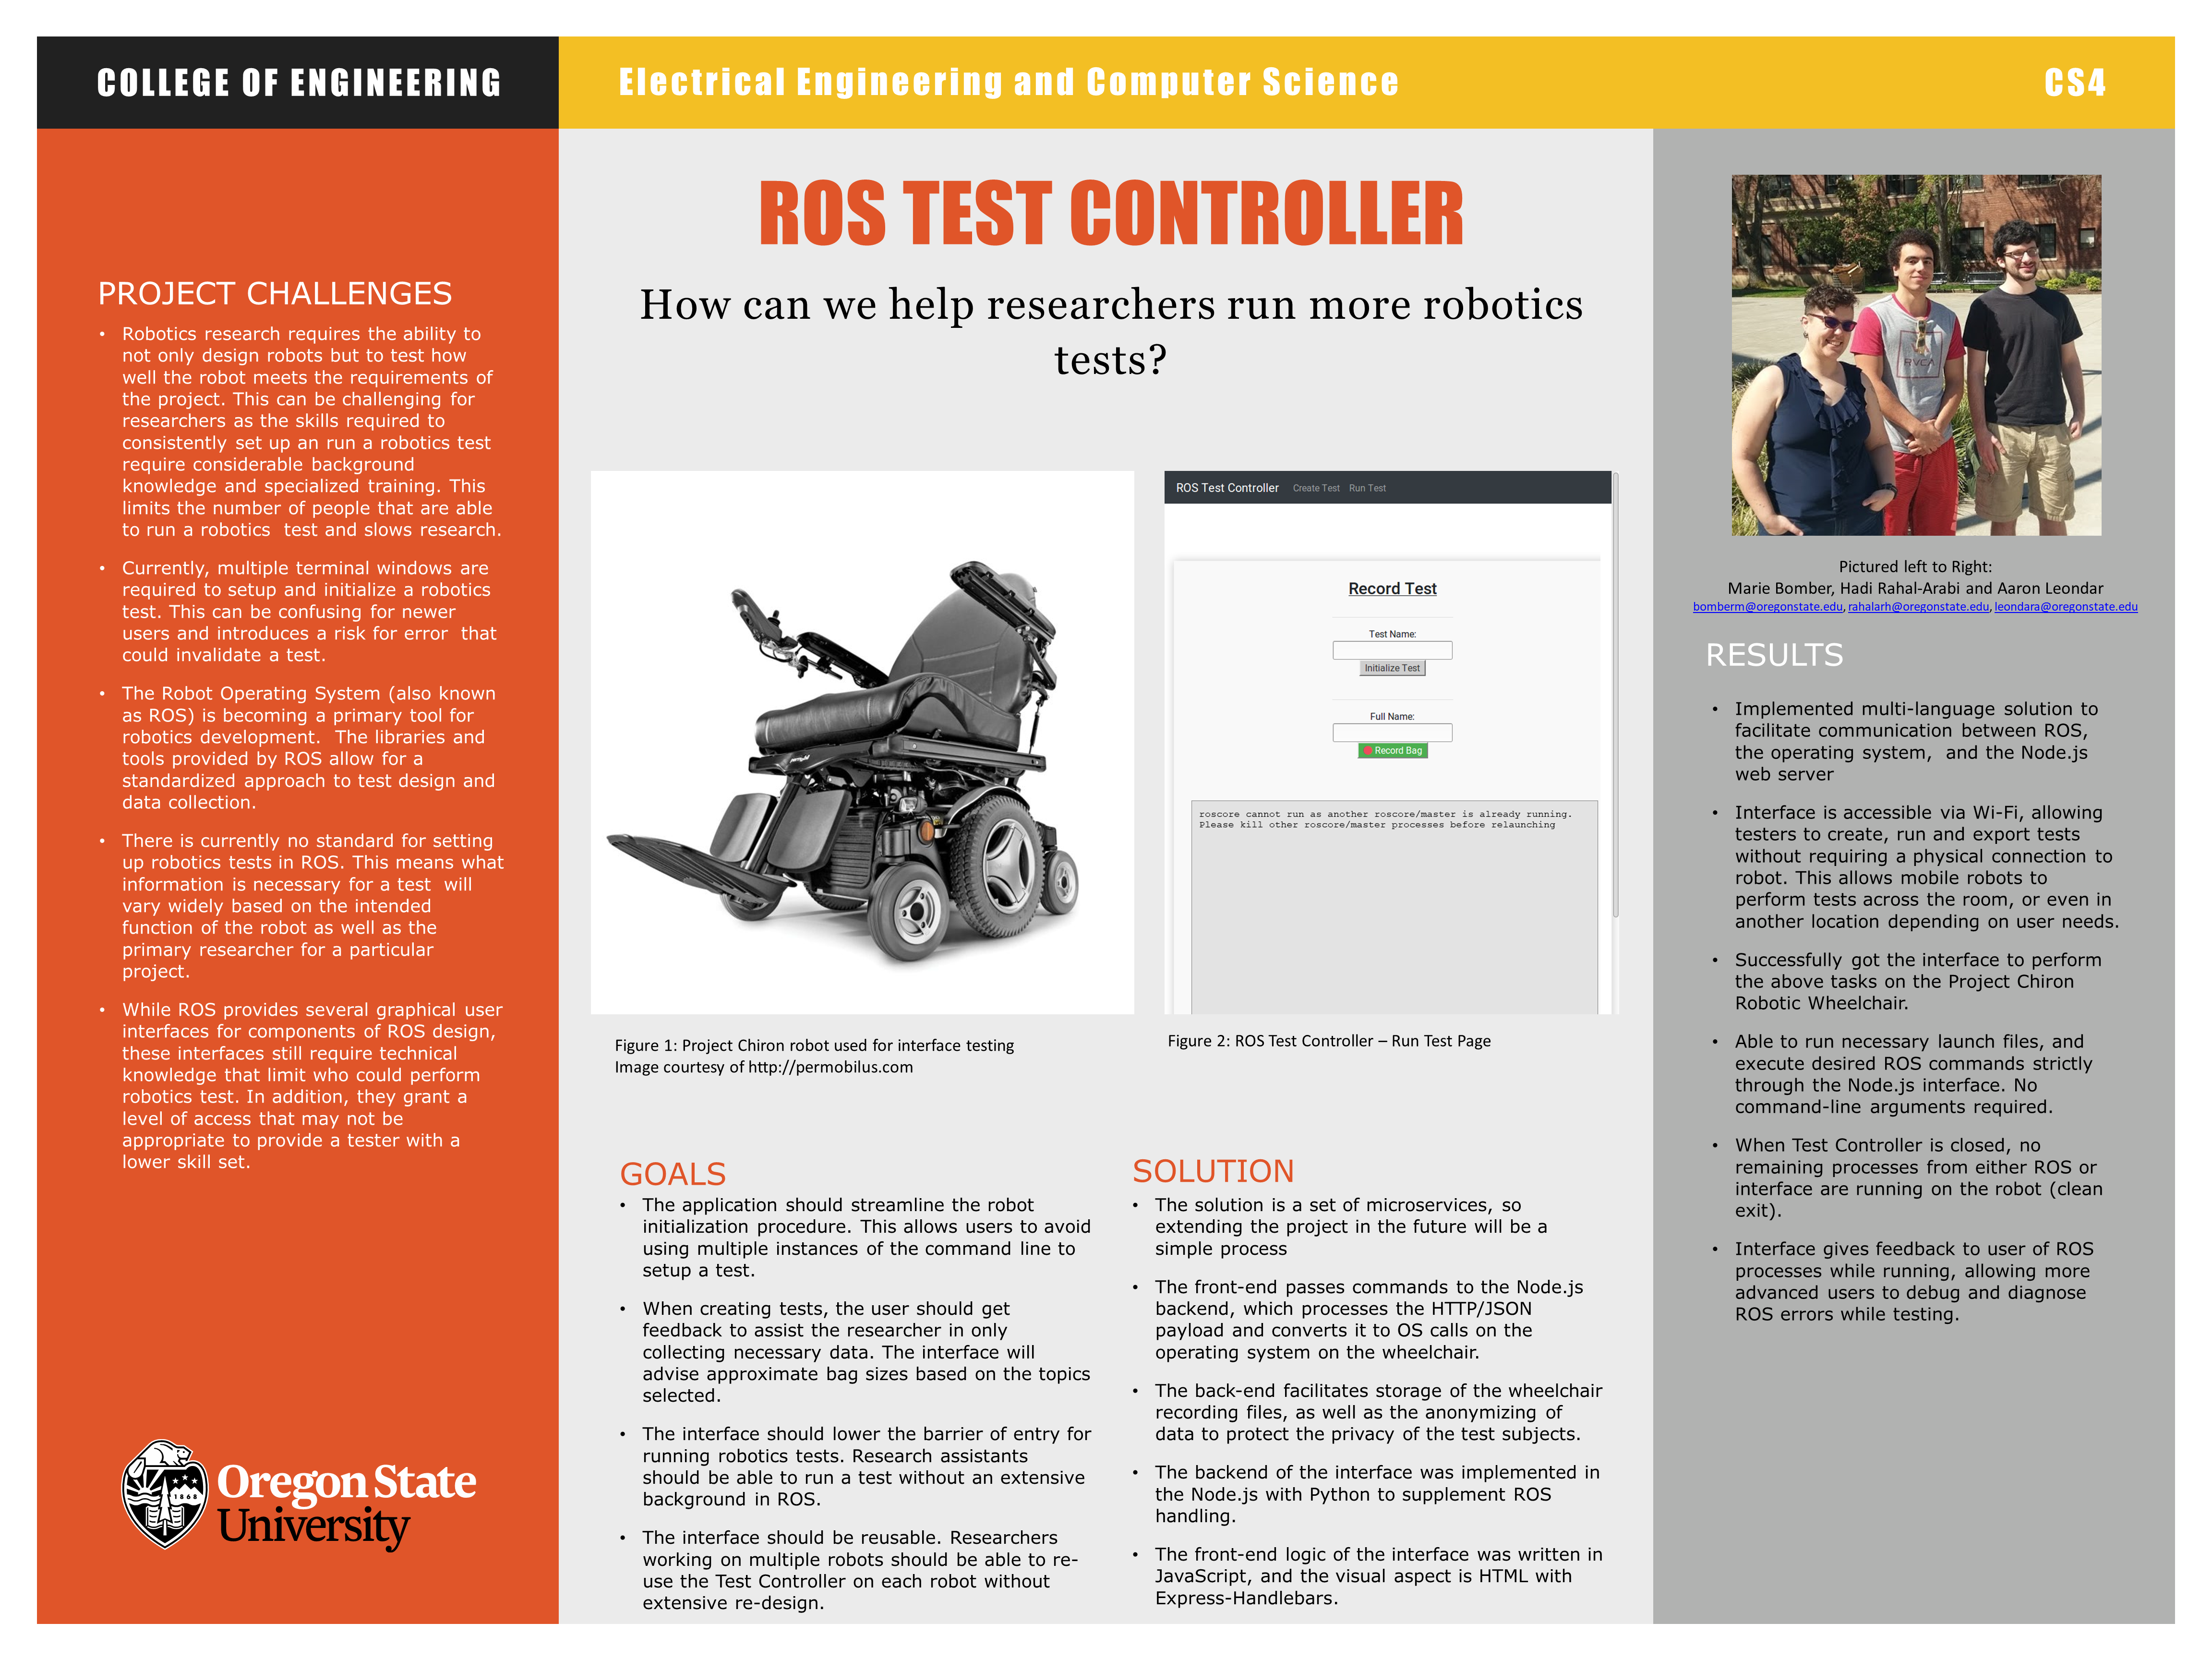
\includegraphics[width=\textwidth]{team04.png}

\chapter{Project Documentation}

\minitoc
\section{Getting Started}


Clone the ROS Test Controller at https://github.com/htrarabi/ROSTestController into a directory on your robot. Ensure your robot has internet access before proceeding with installation.

\section{Prerequisites}

The ROS Test Controller assumes your robot is running Ubuntu 15.10 or higher and has been testing only with ROS Kinetic Kame. While it may work with later ROS distos, it has not been tested and you may get unexpected behavior.

In addition, your robot must have full internet access in order for installation to be successful. After installation, the controller will function without web access, but it's appearance may change slightly.

Because the ROS Test Controller uses both nodeJS and Python 2.7 to control it's behavior, the installer will install these programs if they are not already installed on your robot. In addition, both pip and npm will be installed alongside python and nodeJS.
\section{Installing}

To install the ROS Test Controller, simply run \texttt{sudo -H ./install.sh} in the top level of the ROSTestController directory. This script will confirm that Python 2.7, pip, nodeJS and npm are installed on your robot and install them if not. In addition, install.sh will install several libraries that the Contoller depends on. Once complete, the Test Controller will be ready to run on your robot.
\section{Usage}

To run the ROS Test Controller, ssh into your robot, navigate to your /ROSTestController directory and run \texttt{npm start}. At bootup, the controller will advise that the export server has initialized (typically on port 8080) and that the main controller is running on port 3000. Leave this SSH session running while you use the Test Controller. To use the main controller, enter the robot's IP in a browser window and port 3000.

For example:

\texttt{192.168.0.0.1:3000} would run the controller for a robot with an IP of 192.168.0.0.1.

At this time, the controller will check that roscore is running and you will be taken to the "Run Test" screen.
\subsection{Run a Test}

To run a test, enter the name of the test you wish to run in the "Test Name" field and click "Initialize". Should initialization be successful, you can then enter the name of the test participant and click "Record Bag". Once the test is concluded, click "Stop Bag". While the test is running, a stopwatch will run to advise how long the bag has been recording.

If you wish to change the test that is initialized, simply enter the new test name and click the "Initialize" button again. Similarly, if you wish to record another test, change the test participant name (if needed) and click 'Record Bag' again.

\subsection{Create a test}
To create a test, click "Create Test" on the top bar of the test controller. Give the test a unique name and list any launch files that are necessary to initialize your robot. List launch files using <package name> <filename> (the same format as is used by roslaunch). If you have multiple launch files, separate each package/launch file pair by commas. 

For example, \texttt{controller\_test turtleSim.launch, controller\_test turtleControls.launch} will specify both the turtleSim.launch and turtleControls.launch files for the test being created.

Once the launch files are specified, the 'Test .launch' button can test that all included launch files will successfully run (both on your robot, as well as with the test controller). If the test fails, any error messages will appear on the ssh console that is running the Test Controller. 

After the launch files have been specified, you can add the topics that you wish to be recorded with your test. Similar to the launch files, separate each topic by a comma. Clicking "Estimate Bag Size" will collect a small bag file using the topics you specified and return an estimated Kb/min for each bag recorded in your test. Note, this feature takes approximately 15 seconds to run, during which any modifications to the topics list will not be included in the estimate. 

Once you are satisfied with the settings for your test, click "Submit Test" and the system will create the setup for your new test. 

\subsection{Export Test Results}
To download any bags that have been recorded under a test, enter the robots IP and the port number specified at boot-up (typically 8080) into your browser of choice. This will display the top level directory for all the tests stored on the robot. Select the name of your test and there will be a directory for each test participant for your tests. Names \textit{will} be encrypted in order to meet IRB requirements. Select the directory you wish to export, and you will be able to download the test recording you desire.

\section{Known Bugs}

\begin{itemize}
	\item ROS Test Controller cannot be run as Super User

	\item At this time, there is no checking if a test name has already been used. If a test name is reused, the previous test configuration file will be overwritten.

	\item If the Test Controller crashes, the export server (a separate process) will still run in the background. This process can be killed by using \texttt{pa -a} to get the pid of the server (it will be a node process) and \texttt{sudo kill -2 <pid>} to kill this process. Otherwise, the next instance of Test Controller will use a new port and this can cause multiple file server ports to be open on your robot.

	\item On occasion, the initialize button will become unresponsive. Refresh the page and this behavior will be corrected.
\end{itemize}

\section{Future Enhancement Possibilities}

\begin{itemize}
	\item Change the Test Name field to a drop down of current tests to prevent typos for test name confusion from causing "No Test Found" errors when initializing.

	\item There is infrastructure to allow test participant names to be pre-specified when a test is created. If implemented, "Participant Name" field could be a drop down to prevent name typos from causing tests from the same participant to be stored in separate directories.

	\item Move all ROSHandling functionality from Python calls to nodeJS functions. This would allow the Test Controller to be a pure nodeJS solution and possibly simplify the code base.

	\item Refactor ros.js to improve code clarity and eliminate redundancy.

	\item Because a user must log into a robot in order to start ROS Test Controller, the decision was made for the Test Controller to not have a separate authentication system for the Controller. With that said, the addition of a separate authentication system (and heirarchy to support 'test creator' vs 'authorized tester') could improve the security and enhance usability.
\end{itemize}

\section{Contributing}

Submit pull requests if you have an update that improves the functionality of this Controller and an author or the Project Owner will test and approve changes.

\chapter{Recommended Technical Resources}
\minitoc
\section{ROS Resources}
\begin{itemize}
	\item http://www.ros.org/ - Primary source for debugging ROS errors and exploring ROS libraries.
	\item http://wiki.ros.org/ROS/Tutorials - Setting up/installing ROS
	\item Programming Robots with ROS: A Practical Introduction to the Robot Operating System - Great introduction to ROS systems and played a critical role in understanding what the ROS Controller required to successfully run tests.
\end{itemize}

\chapter{Conclusions and Reflections}
\minitoc
\section{Marie's Reflections}
\subsection{What technical information did you learn?}
Over the course of this project, I gained technical proficiency in three main areas, the Robot Operating System (ROS), nodeJS and finally, general web design. 

From ROS, I gained a basic understanding of the interactions within the Robot Operating system, including how to initialize a robot and record a rosbag. I learned how to create packages using catkin, and how to create and run ROS launch files. In addition, I gained an understanding of how different ROS systems interact with one another, and how to debug ROS output to identify system issues. While I will by no means claim to be even a novice ROS users at this point (as most of my work was not with designing ROS systems, but instead interacting with systems already created); I am now at least able to interact with a robot and do basic debugging. 

For nodeJS, while I had interacted with javascript in the past, it had been almost two years from the last time I had worked with it. It was almost like learning a new language when I first started helping with the core ros.js functionality when we restarted the project mid-way through winter term. At first I was a bit hesitant to dive into node, mostly because I am not a fan of web development. But once the first supplemental functions were created, it was easy to pick up what was necessary for each page call, and build a robust system from there. I was even able to develop callbacks so that the system could more easily give feedback to the user. 

Lastly, web design. During winter term, Aaron and I took Intro to Usability Engineering and the best practices from that class did make it in to the final design. While there are still features and design decisions I would like to add to improve the usability of the Test Controller; the base functionality created is fairly straight forward and clear. From the general aesthetics that Aaron created, I was able to tweak and supplement features to better meet the specifications of our design document and help polish the final product that we delivered to our client. 

\subsection{What non-technical information did you learn?}
The biggest non-technical skills I picked up over the course of this project were mostly related to project management (as I delve into in the next questions), but I also learned a lot about work-life balance. During fall term, even though I felt like a had a good grasp on the scope and requirements of the project, I did not have a good grasp on balancing my stress levels regarding the project needs. Toward the end of fall term this turned into panic attacks when working on the Technical Review and quite a lot of energy spent panicking about both assignments and the success of the project as a whole. It took until Winter term for me to calm down and be able to approach each task with a clear head, and understand that my desires for perfection in each and every portion of this project was not only unreasonable to ask of myself, but also of my teammates. Could more have been done? Perhaps, but our client seems satisfied with our results and that is what is most important. 

\subsection{What have you learned about project work?}
My biggest areas of growth in this project relate to both project work and project management. as previously mentioned, anxiety and work/life balance were major struggles for me at the beginning of the school year. Also difficult for me was finding a compromise between my expectations and the expectations of my teammates. I have always been a perfectionist when it comes to my school work and being able to let go and accept that Aaron and Hadi's contributions were just as good, even if they weren't in my particular style, was a challenge. This led to a bit of stress when documentation was being created and I felt the need to go back and edit so a perfectly fine section of information in  order to meet my standards.

I also learned having a team lead who has a good grasp of each element of the project and the end goal is critical. On the flip side, I also learned that having the entire team have this level of understanding of a project is unrealistic. When you have three individuals working on a team, you'll likely have six different ideas of what the end product will look like. Having one person be in charge of this final goal not only makes sure how each element interacts is understood and taken care of, it also helps prevent a project from spiraling out of control if team members have different ideas how the project should go. 
\subsection{What have you learned about project management?}
The most important lesson I've learned in project management is to know your teammate's strengths and weaknesses and to trust their judgment. We would have moved to a node solution (or even started with a node solution) had I trusted Hadi's recommendations in fall term or early winter. In addition, trusting Hadi's skills in developing the node solution helped us pick up a lot of time that had been lost by my stubbornness.

On the other hand, I also learned to be specific when it came to project goals and requirements, especially when giving directions for a project stage. We had planned to deliver a 'bare-bones' version of the Test Controller during week six of winter term. When hardware issues prevented us from testing and delivering this product to our client, I had said that we shouldn't wait for the hardware issue to be resolved before we moved on to the next project stage. Both Hadi and Aaron agreed and I let the matter be. The following week, I realized nearly no work had been done because they had been waiting on direction from me on where to start with the next project stage. I had assumed they knew in general what their next steps were and because I was not specific, we lost nearly a week of development time. From that point forward, I tried to have a list of actionable items for everyone in the group, to make sure we wouldn't lose more time (though I was not always successful I admit). 
\subsection{What have you learned about working in teams?}
When working in teams, I've learned that I need to let go. Early on in the project I was very controlling and I needed each element of the project to be perfect or I feared ruin. In truth, teams work best if each member has an equal investment and are honest about their goals and desires. Our team dynamic improved a great deal when I took on the management role late into fall term, and it improved even more when I let go a bit and stopped trying to force everything to go exactly my way. 
\subsection{If you could do it all over, what would you do differently?}
It probably comes as no surprise that my biggest 'do-over' would be to start with the right technology from the get go. Had we went with a node solution as recommended by Hadi in Fall term, we would have saved several weeks of development time and been able to show an even more polished final product both at Expo and at the end of this term. I also would have addressed some medical issues sooner, that further hampered the project and led to no small amount of stress. All in all though, I am happy with what we produced. 
\section{Aaron's Reflections}
\subsection{What technical information did you learn?}
\subsection{What non-technical information did you learn?}
\subsection{What have you learned about project work?}
\subsection{What have you learned about project management?}
\subsection{What have you learned about working in teams?}
\subsection{If you could do it all over, what would you do differently?}
\section{Hadi's Reflections}
\subsection{What technical information did you learn?}
\subsection{What non-technical information did you learn?}
\subsection{What have you learned about project work?}
\subsection{What have you learned about project management?}
\subsection{What have you learned about working in teams?}
\subsection{If you could do it all over, what would you do differently?}

\appendix
\minitoc
\section{Essential Code Listings}


\end{document}
